\chapter{Experiments and results}
In the previous chapters we have explored the problem of dissemination of information in distributed
trust systems. We offered a solution in the form of our multichain based TrustChain architecture, extended 
it with internal agent state transparency and designed a mechanism that prevents any free-riding on
dissemination and validation of information on transactions. In this chapter we aim to prove the 
properties of the mechanism and architecture by experimental analysis. We built a proof-of-concept
software that fully implements the architecture and mechanism described in this work. It allows us 
to run an emulation of an agent network and study the behavior of agents in the presence of strategic
manipulators.

\section{Implementation details}
\begin{itemize}
    \item Python implementation 
    \item zermq sockets
\end{itemize}


\section{Experiment design}
The goal of the experimental analysis is to show that free-riding on dissemination and validation of
transaction information is no longer possible with the extension of TrustChain proposed in 
chapter~\ref{chap:state_transparency} and the mechanism in chapter~\ref{chap:mechanism}. This would
be a major step towards a secure and valid distributed trust system. 

In each experiment a small group of agents forms a network. Each agent is acting completely autonomously 
but is aware of the other agents in the network, an assumption that simplifies the experiment. In the
real world agents will not be aware of all other agents but for the sake of exploring the properties
of our mechanism the peer discovery process is not of importance. All agents run a main decision loop
at high frequency and have a small chance of starting an interaction each time step. When starting 
an interaction the agent acts according to the specific version of the software that agent runs. For
the experiments we distinguish different types: 

\begin{itemize}
    \item \textbf{Honest agent}: The honest agent acts exactly according to the rules of the system
    architecture and the mechanism. In the application context this would be a standard installation 
    of the software.
    \item \textbf{Dissemination free-rider}: An agent that performs transactions normally but does
    not respond to exchange requests or start own exchanges.
    \item \textbf{Validation free-rider}: An agent that performs exchanges and transactions normally
    but does not perform any validation
\end{itemize}

With these types of agent we run experiments with different sets of agents. In experiments with only
a single dishonest agent, the experiment is successful if the honest agents stay among themselves
and ignore the dishonest agent. That is, the dishonest agent should have 0 transactions at the end
of the experiment. In the case with multiple dishonest agents we have to make a distinction between
multiple single acting dishonest agents and collaborating groups of dishonest agents. 

\section{Experiment results}
\subsection{Baseline honest}


\begin{figure}[h!]
    \centering
    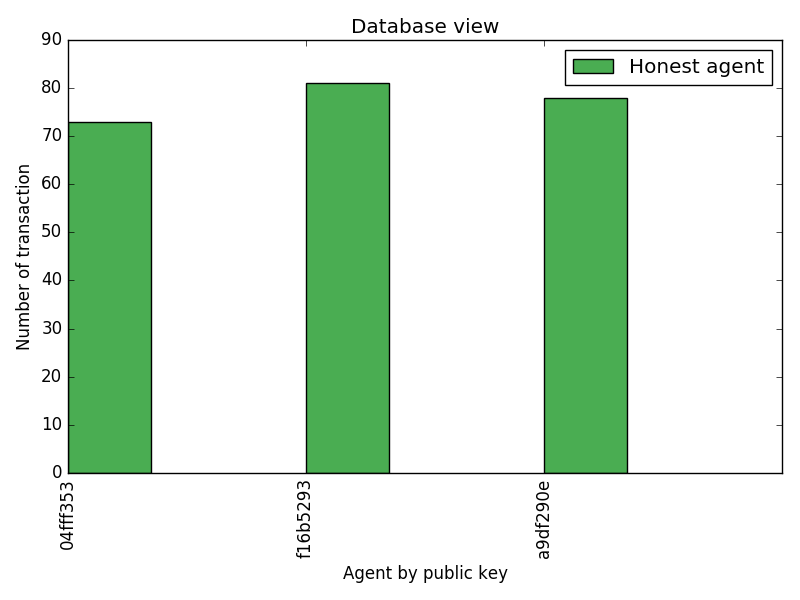
\includegraphics[width=0.7\textwidth]{images/baseline_honest}
    \caption{Baseline experiment with only honest agents}
    \label{baseline_honest}
\end{figure}

\subsection{Single dishonest agent}

\begin{figure}[h!]
    \centering
    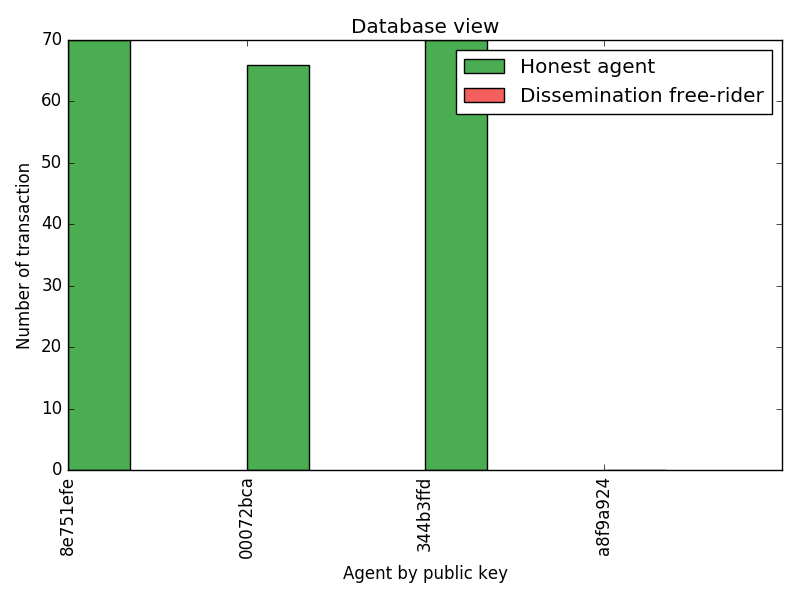
\includegraphics[width=0.7\textwidth]{images/single_dis_free_rider}
    \caption{Baseline experiment with only honest agents}
    \label{baseline_honest}
\end{figure}

\subsection{Collaborating dishonest agents}

\begin{figure}[h!]
    \centering
    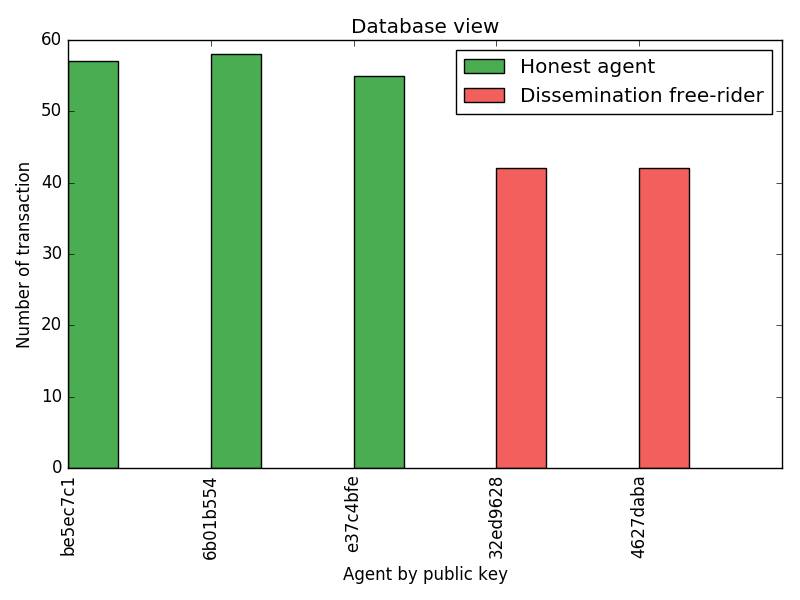
\includegraphics[width=0.7\textwidth]{images/multi_dis_free_rider}
    \caption{Baseline experiment with only honest agents}
    \label{baseline_honest}
\end{figure}

\subsection{Validation free-rider}
{\color{red} TODO}

\section{Application specific experiments}

\subsection{Sybil attack}